
As discussed in the previous subsection, high-precision electroweak
observables are interrelated, and can be combined to predict any
other; deviations from expectations would be evidence for anomalous
interactions contributing to the loop corrections which influence
them.  The mass of the $W$ boson is a signifcant constraint on the
others; historically it has served as a predctive guide in the search for
both the top quark and the Higgs boson.  Now that both of those have been
measured precisely, the situation has reversed, and they can be used
to predict a value for $M_W$ of $80.358 \pm 0.008$
GeV~\cite{Baak:2014ora}, in comparison to the direct experimental
measurement $80.385 \pm 0.015$ GeV~\cite{Aaltonen:2013iut}, motivating
an improvement in precision by at least a factor of two.

The LHC experiments have not yet produced a measurement of the $W$
boson mass, but it is a stated goal of ATLAS, CMS, and LHCb to achieve
precision competitive with the world average.  The statistical
uncertainty of Run 1 data samples should be adequate to achieve this;
CMS analyses of Run 1 data selected over 120 million $W$ candidates
with good signal purity in the muon channel
alone~\cite{Chatrchyan:2013mza,Khachatryan:2016pev},
whereas the best single measurements from the
Tevatron~\cite{Aaltonen:2012bp,Abazov:2012bv} currently use roughly 1
million events each.  The LHC experiments face larger systematic
uncertainty challenges to the Tevatron, however.

The $W$ mass is typically estimated from the lepton $\pt$ or
lepton-$\MET$ transverse mass distributions.  This incomplete
reconstruction introduces modelling uncertainties from PDFs. In
proton-proton collisions at 7 TeV and higher, $W$ production has both
valence quark/sea anti-quark and sea quark/sea anti-quark components,
whereas proton--anti-proton collisions are predominantly valence
quark/valence anti-quark.  The latter are much better constrained
experimentally than the former, and so signifcant progress must be
made on sea quark PDFs to reduce associated $W$ mass uncertainties to
competitive levels.  The LHC W and Z data themselves have been used to
constrain light sea and valence quark PDFs via the $W^+/W^-$
production
asymmetry~\cite{Khachatryan:2016pev,Aaij:2014wba,Chatrchyan:2013mza,Chatrchyan:2012xt,Aad:2011dm}
and lepton rapidity ratio between $W$ and $Z$
bosons~\cite{Aad:2011dm,Aad:2012sb}; Fig.~\ref{fig:ss-precision-wmass-pdf} shows the
precision already acheiveable in these observables compared with
contemporary PDFs.

\begin{figure}[p]
    \centering
    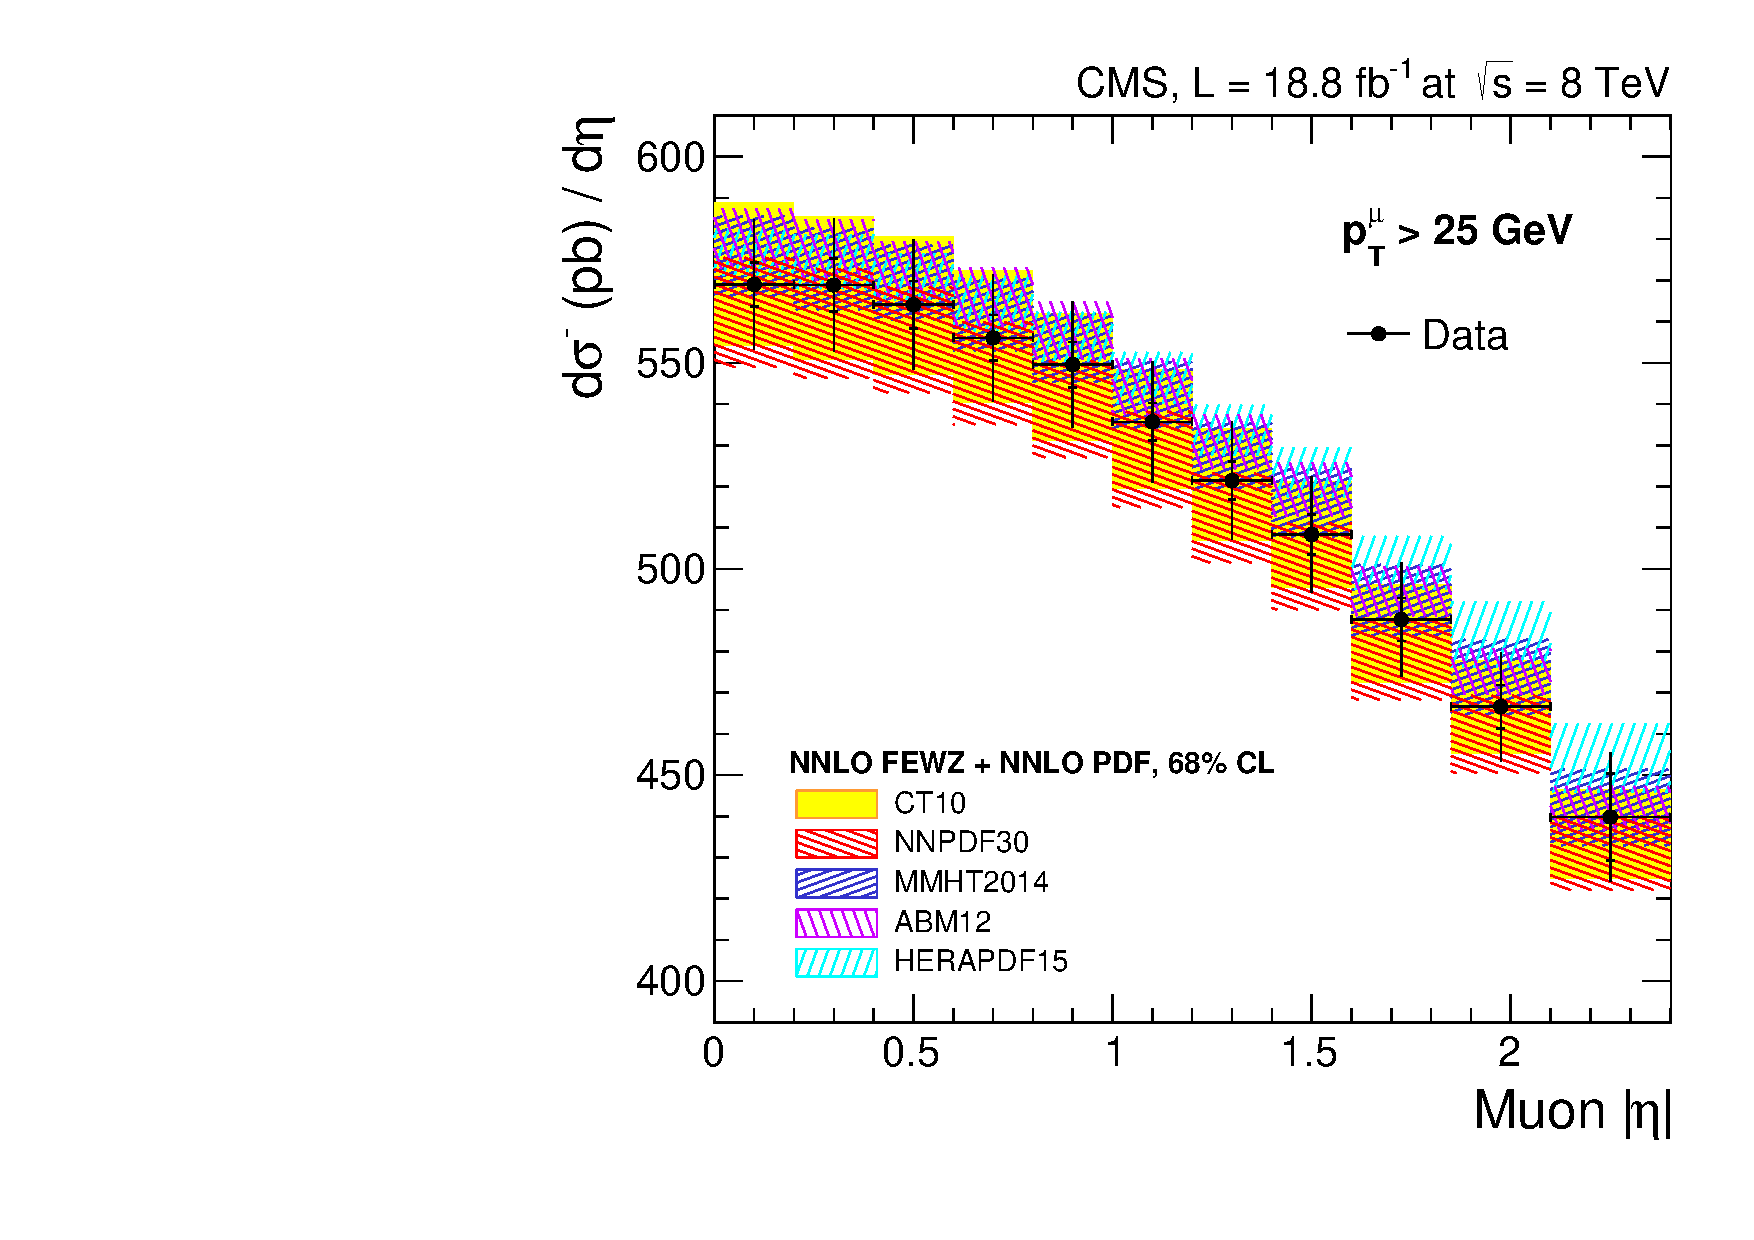
\includegraphics[width=0.45\textwidth]{figures/ss-precision-wmass-wasymmetry.pdf}
    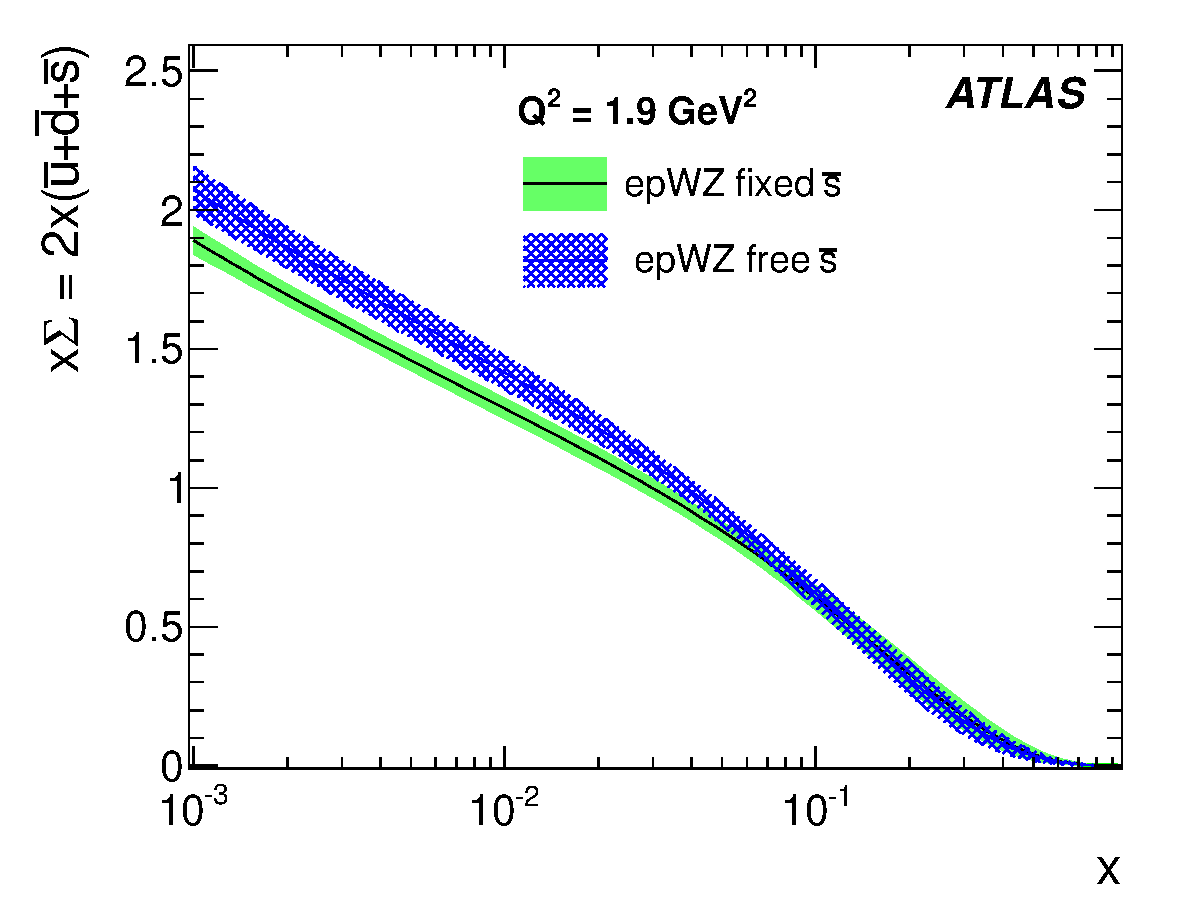
\includegraphics[width=0.45\textwidth]{figures/ss-precision-wmass-wzratio.pdf}
    \caption{
    Left: CMS measurement of the $W$ charge asymmetry at 8 TeV versus lepton
    rapidity, compared with predictions from various PDFs~\cite{Khachatryan:2016pev}.
    Right:  ATLAS constraints on the strange quark PDF from $W$ and $Z$ boson lepton rapidity at 7 TeV~\cite{Aad:2012sb}. 
    .}
    \label{fig:ss-precision-wmass-pdf}
\end{figure}

Another important modelling uncertainty is the $W$ boson transverse
momentum.  This modelling has perturbative, non-perturbative, and PDF
uncertainties. Previous measurements have attempted to constrain these
by precisely measuring the $Z$ boson $\pt$, which constrain underlying
model parameters for both the $W$ and $Z$ spectra, and then translate
those to the $W$ $\pt$ spectrum. 


\begin{figure}[p]
    \centering
    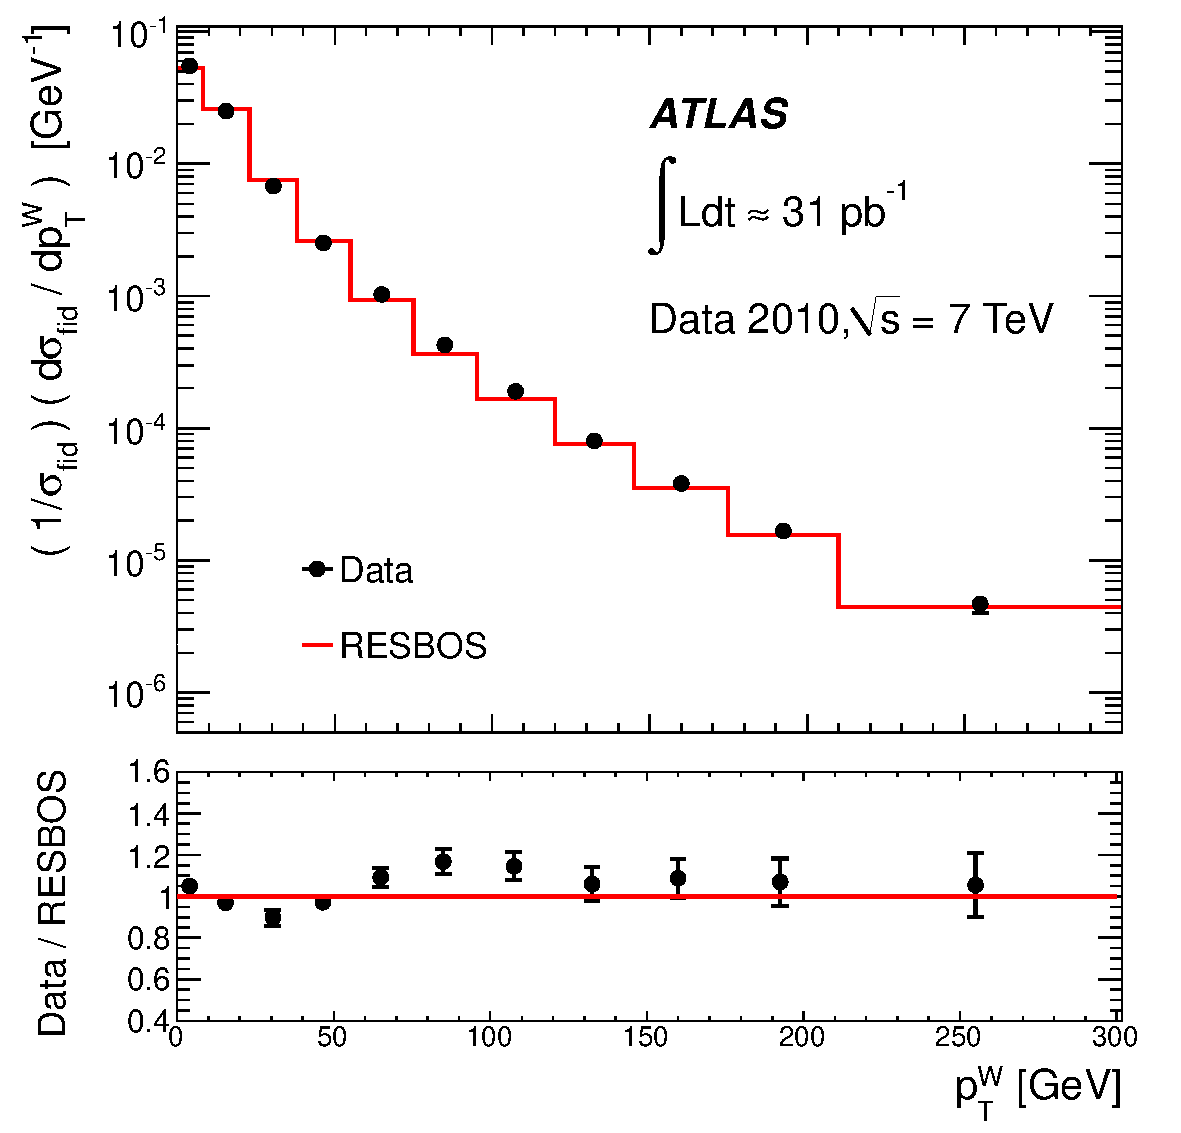
\includegraphics[width=0.45\textwidth]{figures/ss-precision-wmass-wpt-atlas.pdf}
    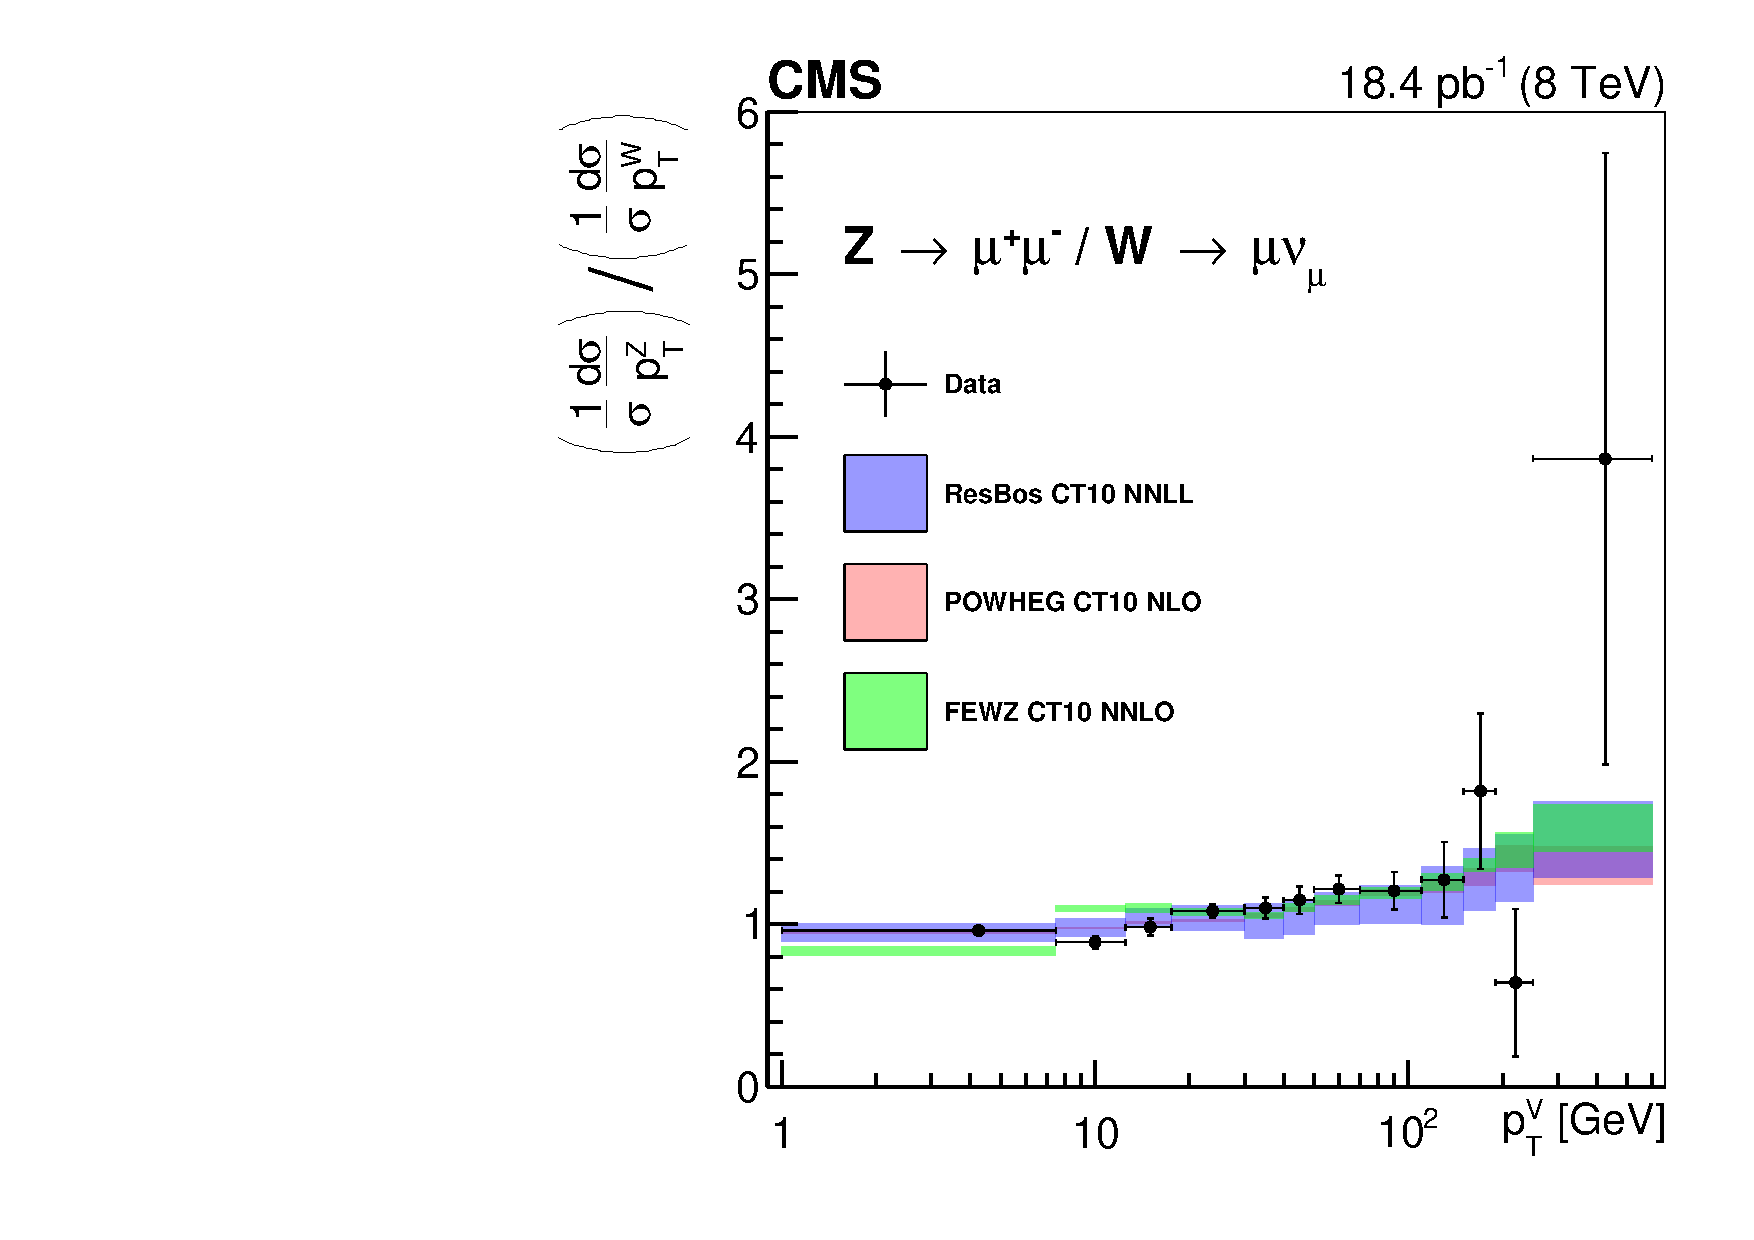
\includegraphics[width=0.45\textwidth]{figures/ss-precision-wmass-wzptratio-cms.pdf}
    \caption{
    Left: $W$ $\pt$ distribution in 7 TeV ATLAS data, compared with predictions~\cite{Aad:2011fp}.
    Right:  Ratio of $Z$ and $W$ normalized differential cross sections with respect to boson transverse momentum in 8 TeV CMS data, compared with predictions~\cite{Khachatryan:2016nbe}. 
}  
    \label{fig:ss-precision-wmass-wpt}
\end{figure}

A related issue is the measurement of $\MET$ in the presence of
pileup.  If transverse mass is to be a competitive observable for
estimating $M_W$ throughout the Run 1 data sample, the resolution must
be competitive in pileup conditions of up to 25 interactions per bunch
crossing.  


%CDF W mass PRD~\cite{Aaltonen:2013vwa}
%CDF W mass PRL~\cite{Aaltonen:2012bp}

%D0 W asymmetry electron~\cite{Abazov:2013dsa}
%D0 W asymmetry muon~\cite{Abazov:2013rja}
%D0 W mass PRD~\cite{D0:2013jba}
%D0 W mass PRL~\cite{Abazov:2012bv}

%CDF+D0 W mass combination~\cite{Aaltonen:2013iut}

%Snowmass electroweak~\cite{Baak:2013fwa}

%Wmass PDF~\cite{Bozzi:2011ww}
